\documentclass[a4paper,10pt]{report}
\usepackage[T1]{fontenc}
\usepackage[table]{xcolor}
\usepackage{titlesec}
\usepackage{graphicx}
\usepackage[inkscapepath=../assets/svg]{svg}
\usepackage{amsmath}
\usepackage{amsthm}
\usepackage{mathtools}
\usepackage{fancyvrb}
\usepackage[english]{babel}
\usepackage{csquotes}
\usepackage{verbatim}
\usepackage{hyperref}
\hypersetup{
   colorlinks=true,
   linkcolor=blue,
   urlcolor=cyan
}
\usepackage{tikz}
\usepackage{amssymb}
\usepackage[sc]{mathpazo}
\linespread{1.05}
\usepackage{microtype}
\usepackage{breqn}
\usepackage{caption}
\usepackage{subcaption}
\usepackage[
   backend=bibtex,%
   bibencoding=utf8,%
   language=english,%
   style=numeric-comp,%
   sorting=nyt,%
   maxbibnames=10,%
   natbib=true%
]{biblatex}
\addbibresource{references.bib}
\usepackage{siunitx}
\usepackage{booktabs}
\usepackage{longtable}
\usepackage{geometry}
\usepackage{multirow}
\graphicspath{ {../assets/img/} }

\newgeometry{hmargin={30mm,30mm}}

% Set TOC depth and sections numbering
\setcounter{tocdepth}{3}
\setcounter{secnumdepth}{3}

% Remove chapters head and reduce spacing
\titleformat{\chapter}[hang]{\Large\bfseries}{\thechapter \hspace{2ex}}{0pt}{\Large}
\titlespacing{\chapter}{0cm}{0cm}{0.5cm}
\usepackage[parfill]{parskip}

% Make quotes italic
\renewcommand{\mkbegdispquote}[2]{\itshape}

% Change texttt line breaks
\renewcommand{\texttt}[1]{%
  \begingroup
  \ttfamily
  \begingroup\lccode`~=`.\lowercase{\endgroup\def~}{.\discretionary{}{}{}}%
  \catcode`/=\active\catcode`[=\active\catcode`.=\active
  \scantokens{#1\noexpand}%
  \endgroup
}

\usepackage{amsmath}
\newcommand{\argmin}{\mathop{\mathrm{argmin}}}  

\begin{document}
\frenchspacing

% First page
\title{
  {{\large{\textsc{Alma Mater Studiorum $\cdot$ University of Bologna}}}}
  \rule{\textwidth}{0.4pt}\vspace{3mm}
  \small{Statistical and Mathematical Methods for Artificial Intelligence}

  \large{\textbf{Blind Signal Separation (BSS) Problem solved with NMF.}}
}

\author{Lorenzo Cellini (\href{mailto:lorenzo.cellini3@studio.unibo.it}{lorenzo.cellini3@studio.unibo.it})}
\date{\today}
\maketitle
\newpage
\tableofcontents
\setcounter{tocdepth}{1}
%\listoffigures
%\listoftables
\newpage


\chapter{Summary}\label{chap:introduction}
Blind signal separation (BSS) is the task of separating a set of source signals from a set of mixed signals, without the aid of information (or with very little information) about the source signals or the mixing process.
An example of BSS problem is the separation of musical instrument tracks when playing together or the most common "cocktail party" example, where a group of people are talking (during a cocktail party) and one wants to follow one of the discussions.
This is in general a very easy task for human brain, although not easy for machines.

In this work, BSS problem has been addressed through Non-negative Matrix Factorization (\textbf{NMF}) technique: a group of algorithms employed in multivariate analysis and linear algebra that shares common traits with clustering techniques.

The given dataset consists of 20 recording tracks each of 1000 time step length. These are recorded by 20 different microphones and contain a mixture of the tracks played by 4 different instruments.
Applying NMF to the given dataset it is possible to separate the musical instruments tracks, and so it is possible to detect how many (and maybe also what kind of) instruments are playing.

Experiments with a different requested number of instruments have been carried out in order to simulate and compare the algorithm behaviour, when the true number of sources is not known.

\chapter{Background theory}\label{chap:background}
Non-negative Matrix Factorization (or Approximation) consists of factorizing a matrix \textbf{X} into two matrices \textbf{W} and \textbf{H}, where all the three matrices have no negative elements.
The non negativity makes these matrices easier to inspect and interpret and sometimes is ineherent to the real problem itself.
NMF can be seen as computing the columns of \textbf{X} as linear combination of the columns of \textbf{W} with coefficient of the combination taken from \textbf{H}:
\begin{equation}
    \vec{x}_i = W\vec{h}_i
\end{equation}
The dimensions of the factor matrices \textbf{W} and \textbf{H} may be significantly lower than those of the original matrix \textbf{X} and this is a very nice property because it makes NMF a powerful technique to be applied to dimensionality reduction and clustering problems.

There are different types of non-negative matrix factorizations:
the different types arise from using different cost functions for measuring the divergence between \textbf{X} and \textbf{WH} and possibly by regularization of the \textbf{W} and/or \textbf{H} matrices.
In this exercise, the given NMF function implements approximation trough Non-negative Least Square (NNLS) algorithm, a type of constrained least squares problem where the coefficients are not allowed to become negative.

The factorization problem in the squared error version of NMF may be stated as: given a matrix \textbf{X} find non-negative matrices \textbf{W} and \textbf{H} that minimize the function
\begin{equation}
    f(W,H) = ||X-WH||_F
\end{equation}
subject to $\textbf{W},\textbf{H} \geq 0$.

After the factorization, the columns of \textbf{W} are the new basis for the column of \textbf{X}, while columns of \textbf{H} can be interpreted as the coordinates of a data point in the basis \textbf{W}.

Making a parallel with respect to clustering techniques, the column of \textbf{W} represents the cluster centroids and so, the number of columns of \textbf{W} is the number of clusters found.

\chapter{Exercise}\label{chap:experiment}
In this exercise I have implemented three different experiment: in the first one I have experimented with different values of \emph{m}, the number of sources to be found (also clusters); 
in the second one, after having fixed \emph{m=4}, I have tried different values for $\tau$, that is the relative difference between two consecutive step of the algorithm, used in order to check for convergence;
in the third one I have used NMF function from sci-kit learn package and compared results of the two algorithms.

Results for the different values of \emph{m} are shown in \ref{fig:m_3}, \ref{fig:m_4} and \ref{fig:m_5}.
\begin{figure}[h]
    \center
    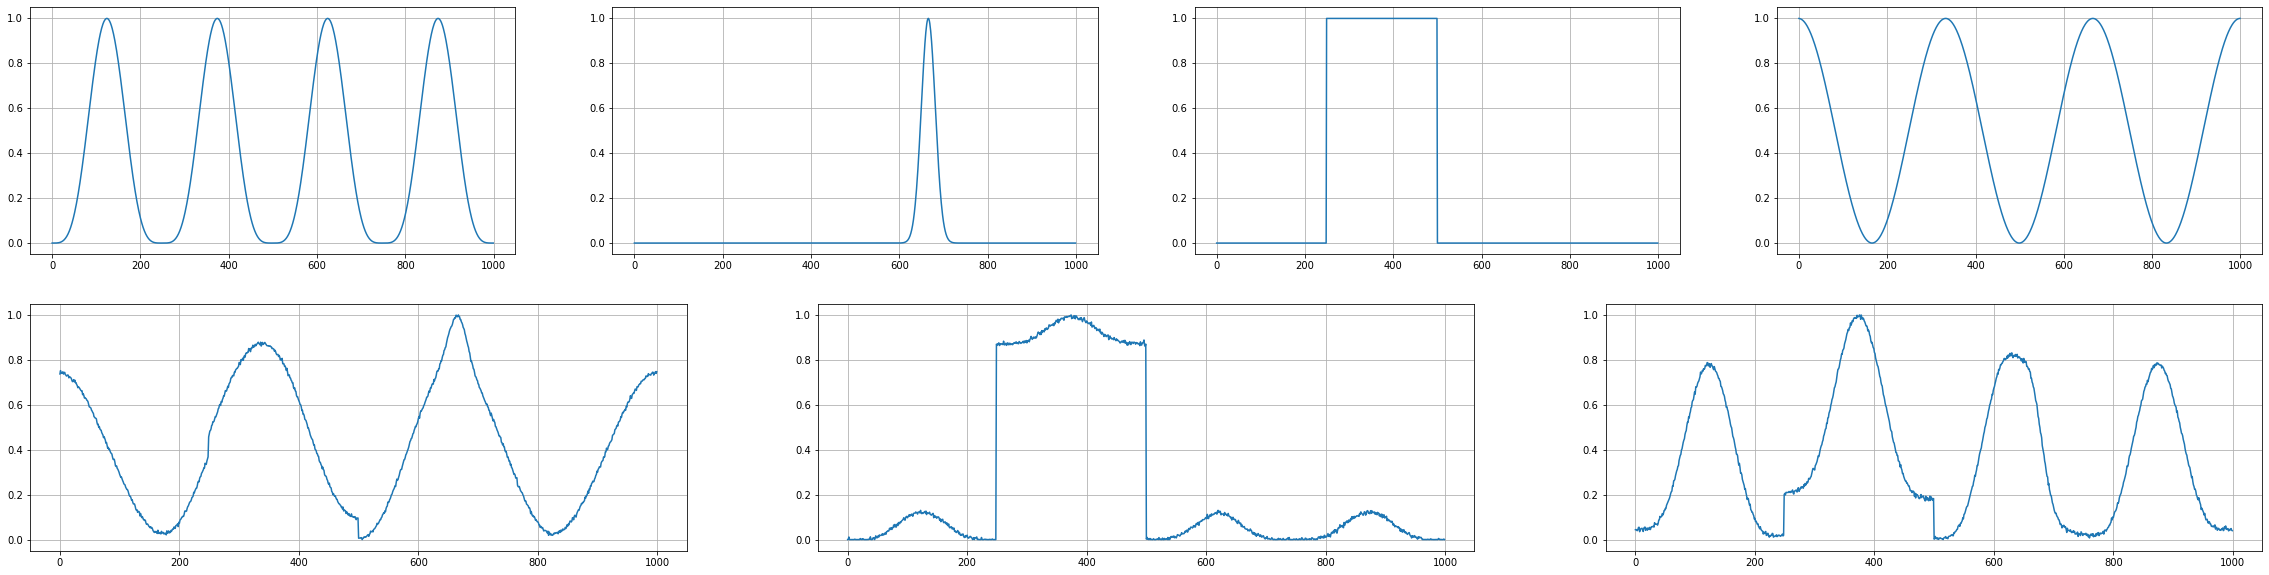
\includegraphics[width=1\linewidth]{nmf_3.png}
    \caption{Source detected with m=3.}
    \label{fig:m_3}
  \end{figure}
  \begin{figure}[h]
    \center
    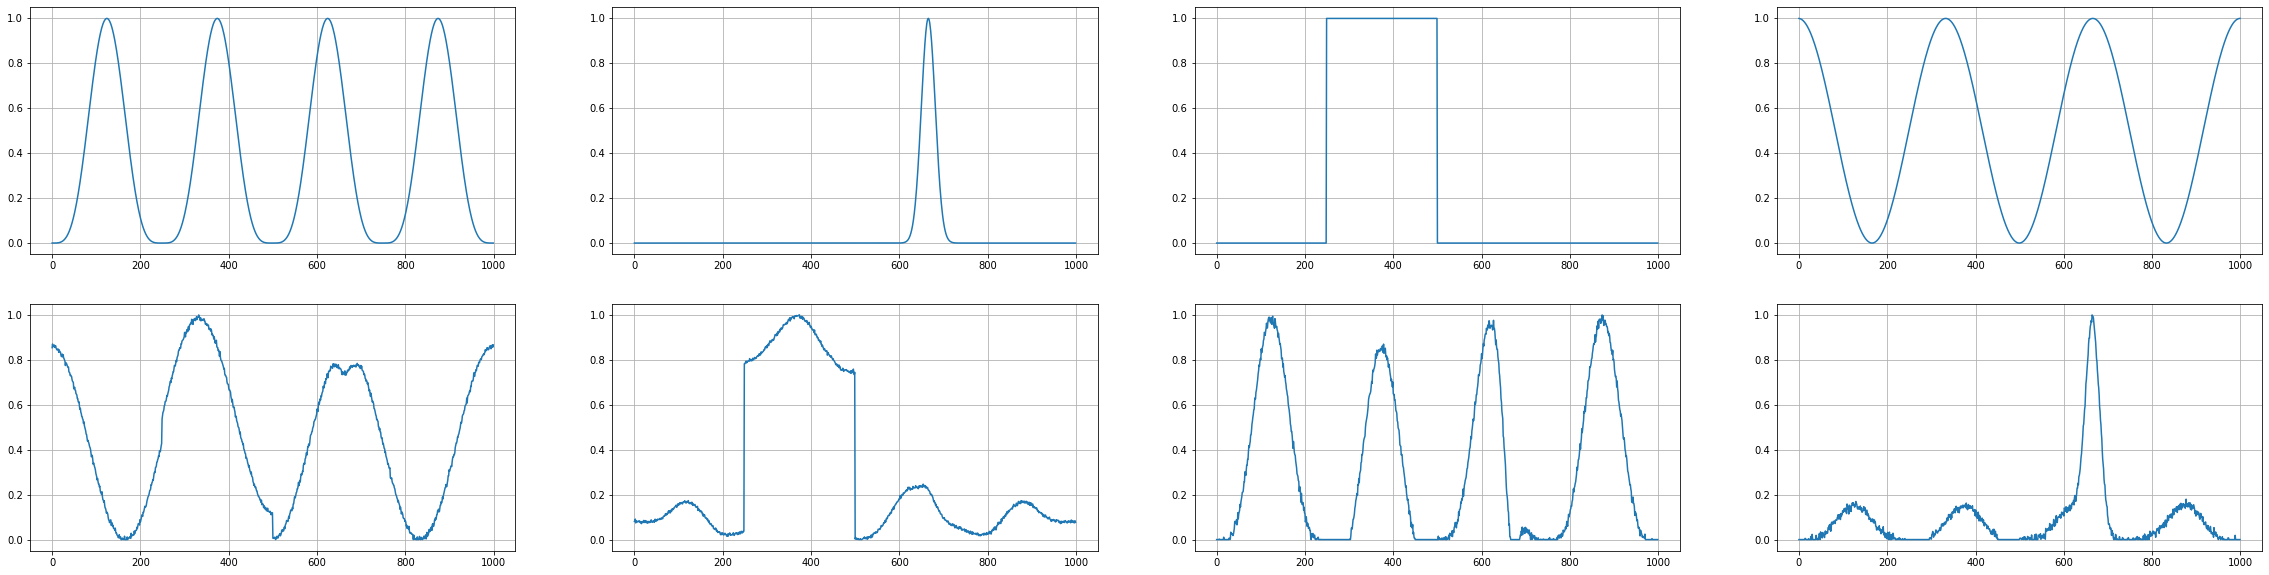
\includegraphics[width=1\linewidth]{nmf_4.png}
    \caption{Source detected with m=4.}
    \label{fig:m_4}
  \end{figure}
  \begin{figure}[h]
    \center
    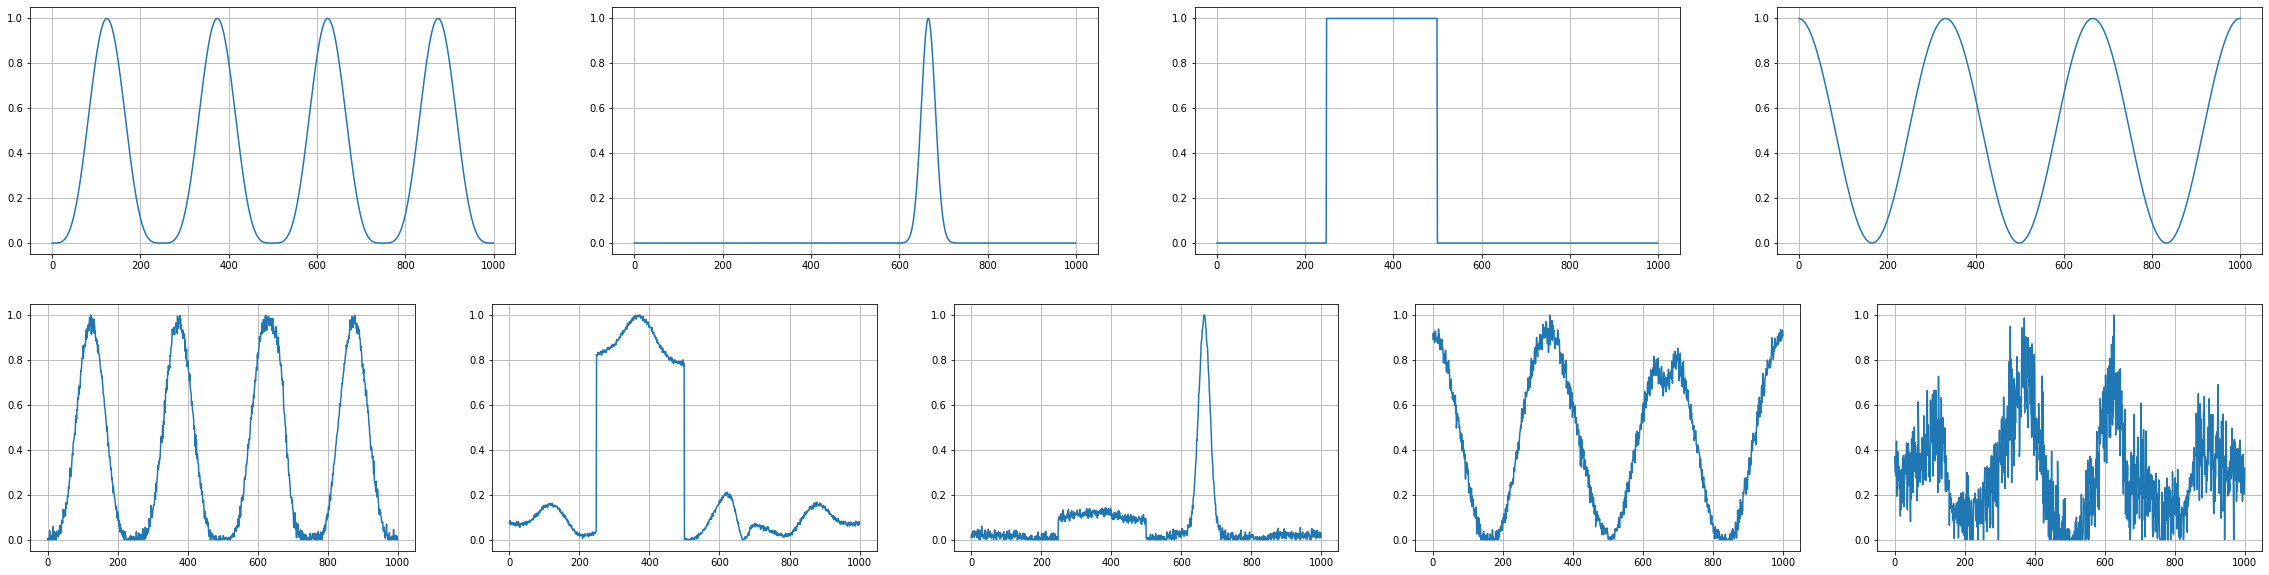
\includegraphics[width=1\linewidth]{nmf_5.png}
    \caption{Source detected with m=5.}
    \label{fig:m_5}
  \end{figure}

As it can be seen, the best result is when m=4, that corresponds to the true number of sources. The ordering of the solution does not matter here because it is always possible to re-arrange matrix column without changing the matrix itself.
In particular, when using a smaller number of sources, it can be observed how the true fourth one is mixed with the detected three, e.g. by looking at the third peak of the first plot.
When asking for 5 sources instead, the algorithm creates a fifth noisy wave and also the other four become more noisy because some points are not assigned anymore to them but they are assigned to the new one.

Now, fixing the number of sources to 4, I tried the same algorithm with the three different values for $\tau$ [1e-2, 1e-3, 1e-4] in order to check how the number of iteration and the approximation error change.
In \ref{fig:nmf_err} it can be seen how the number of iteration increases when $\tau$ becomes smaller: this is quite obvious because the algorithm needs more iteration in order to reach points where the changes between two iteration are smaller than $\tau$.
What is interesting is that the minimum of the reconstruction error, namely the Frobenius norm $||X-WH||_F$, is reached after only 5 iterations. Altough there is no visual difference between the solution after 5 iteration and after 300, from a numerical point of view one should keep the solution that minimize the error and so the one corresponding to the fifth iteration.
In this case, the smallest recostruction error is around 33. 
\begin{figure}[h]
    \center
    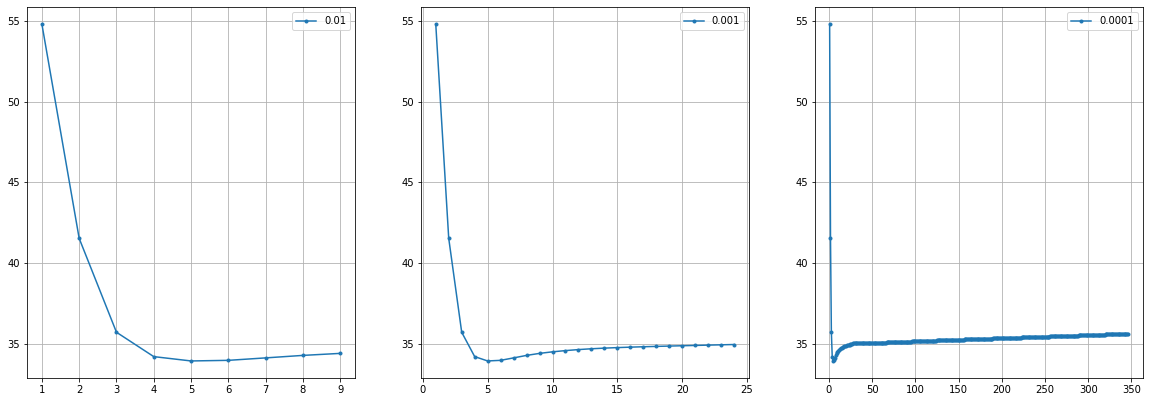
\includegraphics[width=1\linewidth]{nmf_err.png}
    \caption{NMF reconstruction error for different values of $\tau$.}
    \label{fig:nmf_err}
  \end{figure}

Finally, I have run the same experiment using \emph{sci-kit learn} function NMF in order to compare performances of the two algorithm.
The differences in the two NMF functions are in the implemented solver: sci-kit function has the two solvers "cd" for "coordinate descent" and "mu" for "multiplicative update", while the provided custom function relies on non-negative least square algorithm.
All the three are iterative optimization algorithms. 

In \ref{fig:sknmf_err} it can be seen that sci-kit implementation outperform the custom one, and that coordinate descent method is more effective than multiplicative update: indeed the first reaches a better minimum of around 2.5 within 264 iteration, with respect to the latter that reaches a minimum of 2.9 after 269 iterations.
\begin{figure}[h]
    \center
    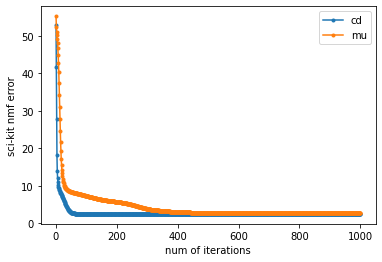
\includegraphics[width=0.6\linewidth]{sknmf_err.png}
    \caption{Sci-kit NMF reconstruction error for different solvers.}
    \label{fig:sknmf_err}
\end{figure}
While sci-kit implementation shows a smaller reconstruction error, the visual inspection of detected sources is not as good as for the custom NMF.
\begin{figure}[h]
    \center
    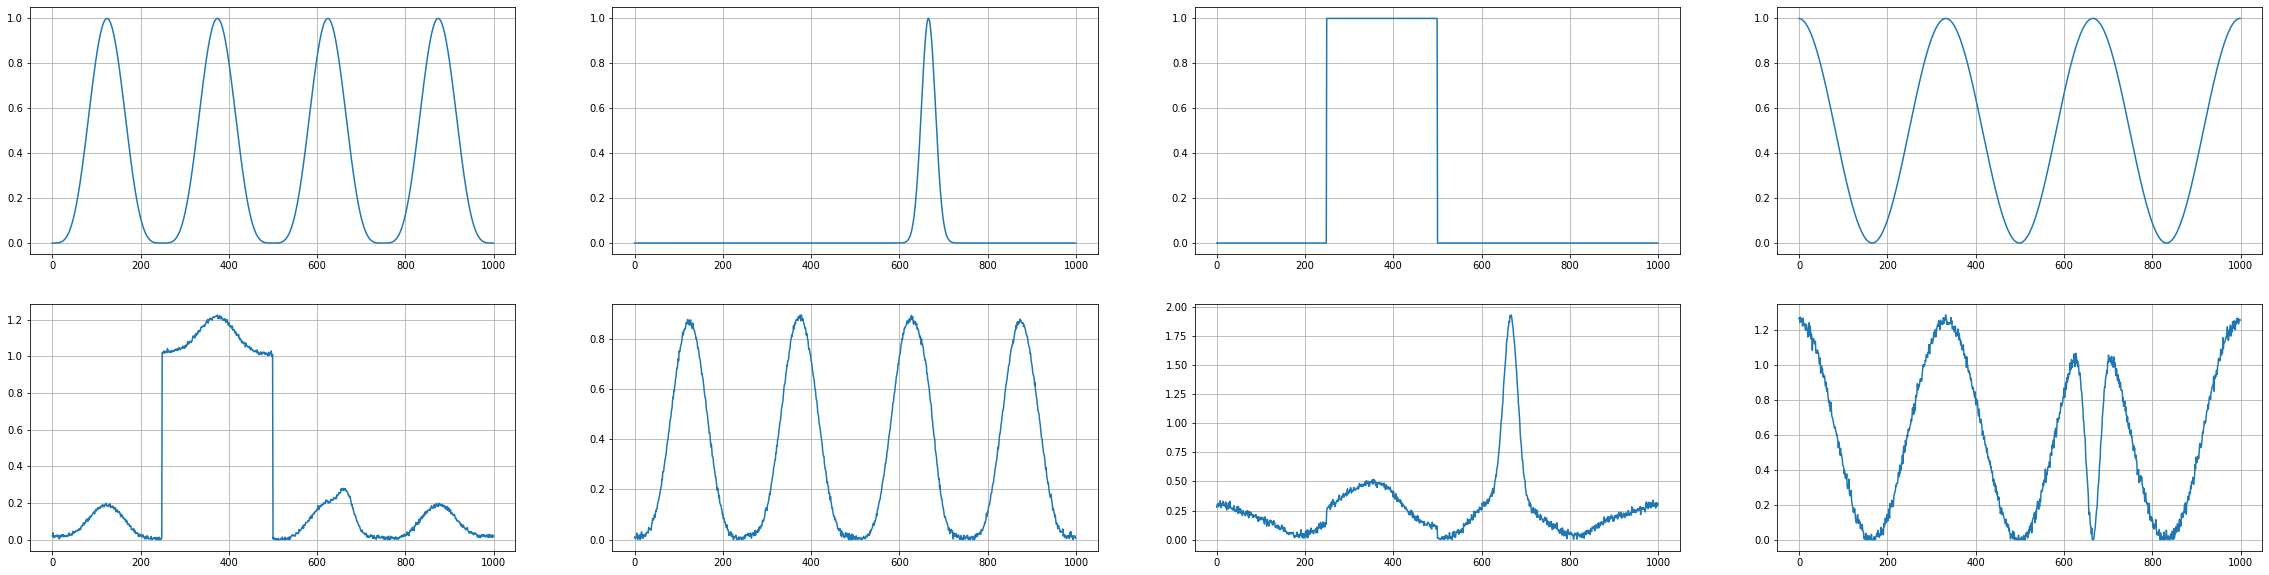
\includegraphics[width=1\linewidth]{sknmf_cd_4.png}
    \caption{Sci-kit NMF source detected for solver "cd".}
    \label{fig:sknmf_cd_4}
\end{figure}

\chapter{Conclusion}\label{chap:conclusion}
NMF has proven to be very powerful in clustering and dimensionality reduction problems like image or sound signal separation, topic extraction in text mining and so on.
As shown in the different experiment, there are a lot of parameters to take into account when running NMF and so, as usual in machine learning, the best approach would be to perform a search grid on the space of parameters in order to find the best configuration for each problem.

Being clustering tipically an unsupervised techniques, the number of sources to be detected is not known in principle and so the procedure should be to try for different values of input \emph{m} and asses results both visually and trough the definition of a fitness function (like in K-means clustering). 

\end{document}
